\item \textbf{{[}HCI/PRELIM/9569/2021/P2/Q4{]}}

Name your Jupyter Notebook as 

\texttt{TASK4\_<your name>\_<centre number>\_<index number>.ipynb }

The task is to write program code for a Tic-Tac-Toe-Tomek game for
two players. 

Tic-Tac-Toe-Tomek is a game played on a 4 x 4 square board. The board
starts empty, except that a single 'T' symbol may appear in one of
the 16 squares. There are two players: X and O. They take turns to
make moves, with X starting. In each move a player puts her symbol
in one of the empty squares. Player X's symbol is \texttt{'X'}, and
player O's symbol is \texttt{'O'}. 

After a player's move, if there is a row, column or a diagonal containing
4 of that player's symbols, or containing 3 of her symbols and the
\texttt{'T'} symbol, she wins and the game ends. Otherwise the game
continues with the other player's move. If all of the fields are filled
with symbols and nobody won, the game ends in a draw. 

Given the 4 x 4 board description containing \texttt{'X'}, \texttt{'O'},
\texttt{'T'} and \texttt{'.'} characters (where \texttt{'.'} represents
an empty square). The following examples show the various winning
positions. 
\begin{center}
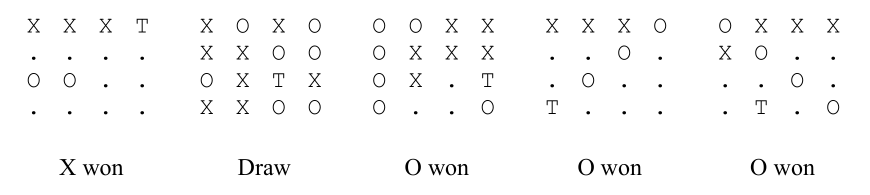
\includegraphics[width=0.5\paperwidth]{C:/Users/Admin/Desktop/Github/question_bank/LyX/static/img/9569-HCI-2021-P2-Q4}
\par\end{center}

For each of the sub-tasks, add a comment statement at the beginning
of the code using the hash symbol \textquoteleft \texttt{\#}\textquoteright ,
to indicate the sub-task the program code belongs to, for example: 
\noindent \begin{center}
\begin{tabular}{c|l|}
\cline{2-2} 
\multirow{2}{*}{\texttt{In{[}1{]}:}} & \texttt{\# Task 4.1}\tabularnewline
 & \texttt{Program Code}\tabularnewline
\cline{2-2} 
\multirow{2}{*}{\texttt{In{[}2{]}:}} & \texttt{\# Task 4.2}\tabularnewline
 & \texttt{Program Code}\tabularnewline
\cline{2-2} 
\multirow{2}{*}{\texttt{In{[}3{]}:}} & \texttt{\# Task 4.3}\tabularnewline
 & \texttt{Program Code}\tabularnewline
\cline{2-2} 
\texttt{In{[}4{]}:} & \texttt{\# Task 4.4}\tabularnewline
 & \texttt{Program Code}\tabularnewline
\cline{2-2} 
\texttt{In{[}5{]}:} & \texttt{\# Task 4.5}\tabularnewline
 & \texttt{Program Code}\tabularnewline
\cline{2-2} 
\multicolumn{1}{c}{} & \multicolumn{1}{l}{\texttt{Output:}}\tabularnewline
\end{tabular}
\par\end{center}

\subsubsection*{Task 4.1 }

Write program code to: 
\begin{itemize}
\item initialize the data structure to represent the 4 x 4 square board,
using the identifier \texttt{board} 
\item generate a pair of random numbers between 1 and 4 
\item place \texttt{'T'} at that random position on the board \hfill{}{[}3{]}
\end{itemize}

\subsubsection*{Task 4.2 }

Write a function \texttt{displayBoard} that will display the game
board clearly to the players. You should use the \texttt{board} as
a parameter in \texttt{displayBoard}. \hfill{}{[}2{]}

\subsubsection*{Task 4.3 }

Write a function \texttt{getPlayerMove} to get players to make their
move (by marking \texttt{'X'} or \texttt{'O'}) on the board. You should
include validation on player\textquoteright s input and check that
the space is not already occupied. Use \texttt{board} as a parameter.
You may include any other suitable parameters. \hfill{}{[}4{]}

\subsubsection*{Task 4.4 }

Write a function \texttt{checkWin} that checks all the conditions
for winning a game and returns \texttt{True} if a player has won the
game, otherwise returns \texttt{False}. Use \texttt{board} as a parameter.
You may include any other suitable parameters. \hfill{} {[}5{]}

\subsubsection*{Task 4.5 }

Write a \texttt{main} function that makes use of the identifiers and
functions from Task 4.1 to Task 4.4 and allows two players, X and
O, to play a game of Tic-Tac-Toe-Tomek. 

The \texttt{main} function should include the following: 
\begin{itemize}
\item display the initial game board with the single \texttt{'T}' displayed
in it 
\item start with player X to make the first move 
\item ensure players X and O take turns to make their move 
\item display the game board after every move made by a player 
\item check for winner 
\item display message on which player has won the game or whether the game
ends in a draw. \hfill{} {[}7{]}
\end{itemize}
Run your \texttt{main} function and produce outputs of \textbf{three}
games where player X wins one game, player O wins another game, and
a drawn game. 

Copy and paste all outputs in a text file as 

\texttt{TASK4\_5\_<your name>\_<centre number>\_<index number>.txt}
\hfill{} {[}3{]}

Save your Jupyter Notebook for Task 4.